\section{Basic Background in Formal Concept Analysis\label{sec:background_fca}}
In this section, we briefly recall some basic background in FCA. 
We focus on the finite case of FCA (with a finite set of objects and attributes) because we want to apply FCA to analyze finite data.
For further details see, \eg, \cite{formal:1999:bernhard,fca-images:2017:ignatov}.

\subsection{Formal Contexts and Formal Concepts \label{sec:fc}}
A \textit{formal context} (FC) is a triple $\langle A, O, \mathbf{I}\rangle $,
where $A$ is a finite set of attributes, $O$ is  a finite set of objects,
and $\mathbf{I} \subseteq A \times O$ is an incidence relation between $A$ and $O$.
%We write the number of attributes as $|A|$ and the number of objects as $|O|$.
A formal context can be represented by binary table $C$ with objects as rows $C_{o}$ and attributes as columns $C_{a}$, for $o\in O$ and $a\in A$.
The entry of $C$ corresponding to $o$ and $a$ is defined by $C_{o,a}=1$ if $(o,a)\in \mathbf{I}$, and $0$ otherwise.
In FCA, entries equal to 1 are also called \textit{crosses}.
\cref{fig:context} is an example of a formal context of shapes and their geometrical properties.
%For simplicity we will use \textit{formal context} to designate $C$ in the rest of the paper.

It is well known~\cite{formal:1999:bernhard} that every formal context $\langle A, O, \mathbf{I}\rangle $ induces a Galois connection between objects and attributes, called \textit{closure operator}: for $X\subseteq O$ and $Y\subseteq A$, defined by:
$X' = \{ y\in A~|~ (x, y) \in \mathbf{I} \textrm{ for all } x\in X \}$ and
$Y' = \{ x\in O~|~ (x, y) \in \mathbf{I} \textrm{ for all } y\in Y \}$.
A \textit{formal concept} is then a pair $(X,Y)$ such that $X'=Y$ and $Y'=X$,  called respectively the {\it intent} and the {\it extent}. 
It should be noticed that both $X$ and $Y$ are closed sets, i.e.,  $X=X''$ and $Y=Y''$.
We denote by $I \subseteq 2^A$ the set of intents, $E \subseteq 2^O$ the set of extents and $C \subseteq I\times E$ the set of concepts.
%
In simple terms, a formal concept is a ``rectangle'' of crosses in a formal context, relating the attributes shared by a set of objects and the objects containing the set of attributes.

\subsection{Formal Concept Lattices\label{sec:lattice}}
The set of all formal concepts can be ordered by inclusion of the extents or, dually, by the reversed inclusion of the intents.
The order relation $\leq$ on concepts is defined as $\langle i_1, e_1\rangle \leq \langle i_2, e_2\rangle \iff e_1 \subseteq e_2$.
As $\leq$ is a partial order relation, the set of formal concepts together $\leq$ form a \textit{partially ordered set}.
More specifically, they form a lattice $L$ called a \textit{formal concept lattice}.

%The lattice formed by the set of formal concepts and the corresponding order relation $\leq$ form a \textit{partially ordered set}.
In lattices, every pair of elements (formal concepts in our case) have a unique \textit{supremum} (or \textit{join}), which is the lowest element which is greater than or equal to the elements in the pair. As such, it is also called \textit{least upper bound}.
Similarly, every pair of elements has a unique \textit{infimum} (or \textit{meet} or \textit{greatest lower bound}).
Additionally, in the finite case that interests us, there exist two special elements in every lattice: \textit{top} (written $\top$) and \textit{bottom} ($\bot$).
$\top$ is the \textit{global maximum} and $\bot$ the \textit{global minimum} of the lattice.
As such, for every concept $c \in C$ in the lattice, we have $\bot \leq c \leq \top$.
Typically, the intent of $\top$ is empty and its extent is $O$, while the extent of $\bot$ is empty and its intent is $A$.

The \textit{strict order relation} $<$ of the order relation $\leq$ is defined by $x < y$ if $x \leq y$ and $x \neq y$.
The \textit{cover relation} $\prec$ is defined by $x \prec y$ if $x < y$ and there is no $z$ such that $x < z < y$.
The \textit{Hasse diagram}, the graph of this $\prec$ relation, is a standard representation for formal concept lattices.
It is an \textit{acyclic directed graph}.
\cref{fig:hasse} is the Hasse diagram of the example lattice from \cref{fig:context}.

%In terms of relations, $<$ is the \textit{reflexive reduction} of $\leq$, while $\prec$ is the \textit{transitive reduction} of $<$ and the \textit{reflexive transitive reduction} of $\leq$.
%Conversely, $<$ is the \textit{transitive closure} of $\prec$.

\begin{figure}
    \centering
        {$\begin{array}{rcccc}
            &\rotatebox{90}{4 sides} & \rotatebox{90}{3 sides} & \rotatebox{90}{Regular} & \rotatebox{90}{Isosceles} \\
            \text{Square} & \times & & \times & \\
            \text{Rectangle} & \times & & & \\
            \text{Rectangle Triangle} & & \times & & \\
            \text{Isosceles Triangle} & & \times &  & \times\\
            \text{Equilateral Triangle} & & \times & \times & \times\\%[4em]
        \end{array}$}
    \caption{Example of a formal context of geometrical shapes.\label{fig:context}}
\end{figure}

\begin{figure}
    \centering
    {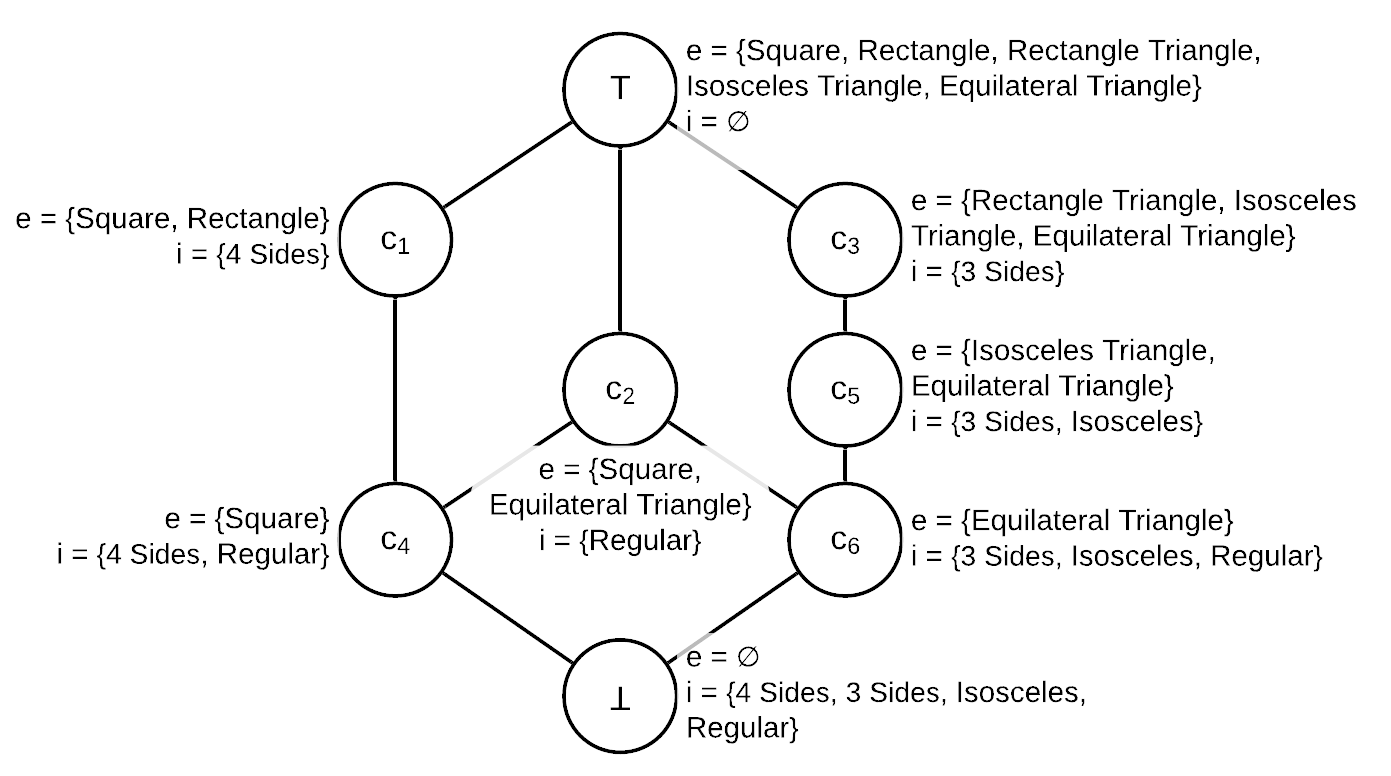
\includegraphics[keepaspectratio, width=\textwidth]{Figures/Ch0/example_full.png}}
    \caption{Lattice of the example context from \cref{fig:context}.}
    \label{fig:hasse}
\end{figure}

% \begin{figure}
%     \centering
%     \subcaptionbox{Context\label{fig:context}}{\scalebox{.8}{
%     %\subcaptionbox{Context\label{fig:context}}{\scalebox{1}{
%         $\begin{array}{rcccc}
%             &\rotatebox{90}{4 sides} & \rotatebox{90}{3 sides} & \rotatebox{90}{Regular} & \rotatebox{90}{Isosceles} \\
%             \text{Square} & \times & & \times & \\
%             \text{Rectangle} & \times & & & \\
%             \text{Rectangle Triangle} & & \times & & \\
%             \text{Isosceles Triangle} & & \times &  & \times\\
%             \text{Equilateral Triangle} & & \times & \times & \times\\%[4em]
%         \end{array}$}}
%     \subcaptionbox{Lattice\label{fig:hasse}}{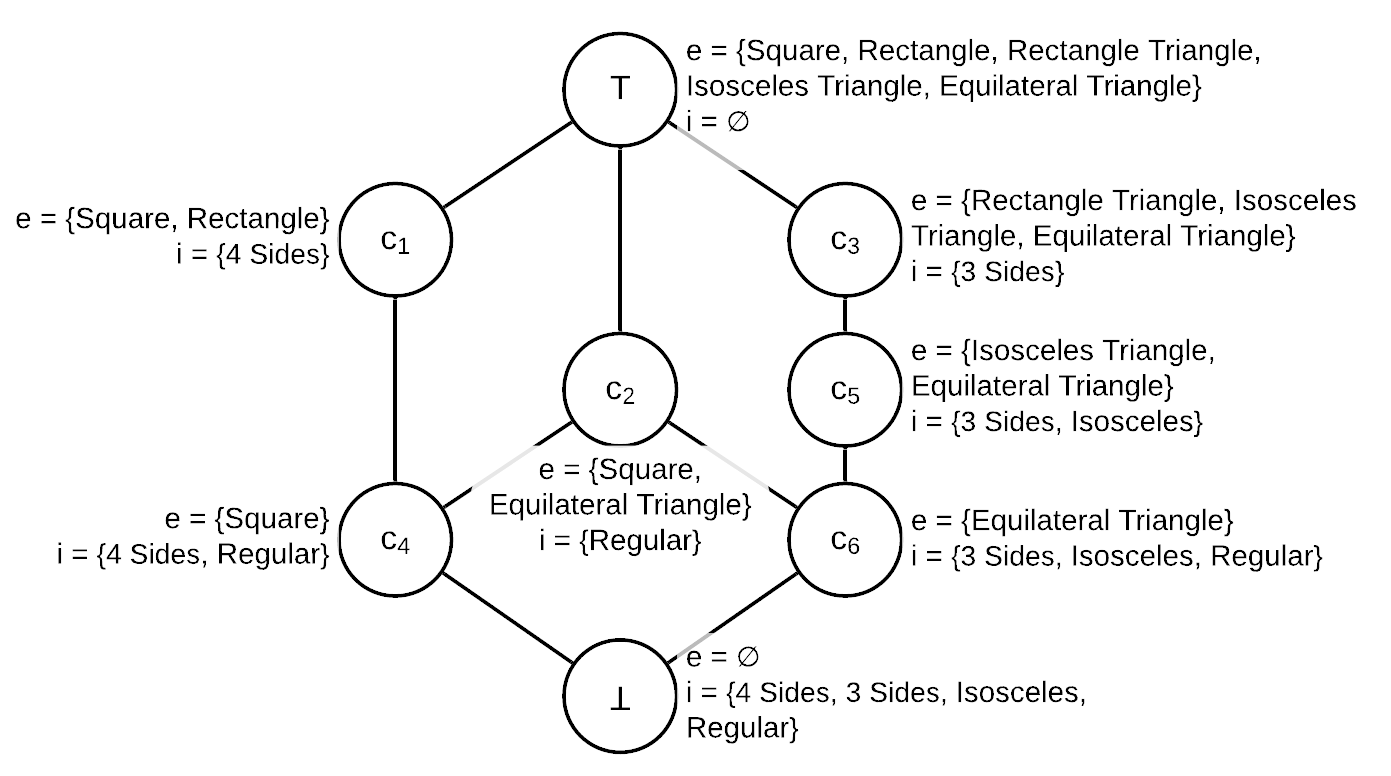
\includegraphics[keepaspectratio, width=.61\textwidth]{Figures/Ch0/example_full.png}}
%     %\subcaptionbox{Lattice\label{fig:hasse}}{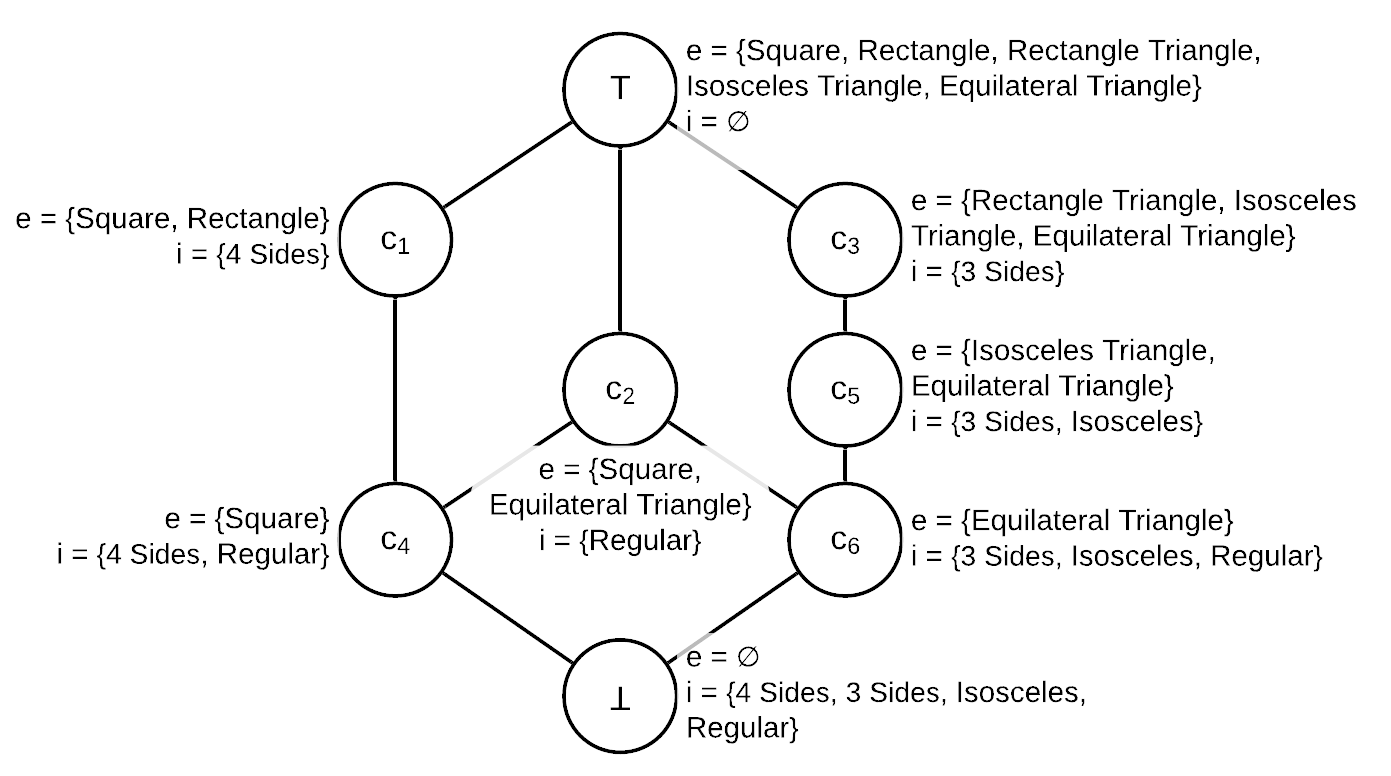
\includegraphics[keepaspectratio, width=.9\textwidth]{Figures/Ch0/example_full.png}}
%     \caption{Example of a formal context and the corresponding formal concept lattice.}
%     \label{fig:lattice-ex}
% \end{figure}

\subsection{Formal Concept Lattices Generation Algorithms\label{sec:lattice-algo}}
A naive way to generate concept lattices is to follow the definition of formal concepts.
The first step is to compute either the intents or the extents, and use it to build the set of formal concepts.
To achieve this, we can construct the set of extents as $E = \{Y'' \textrm{ for all } Y\in2^O\}$ and the set of concepts $\{\langle e', e\rangle \textrm{ for all } e \in E\}$.
The set of intents would be $I = \{X'' \textrm{ for all } X\in2^A\}$ and the set of concepts $\{\langle i, i'\rangle \textrm{ for all } i \in I\}$.
The number of possible extents and intents are respectively $|2^O| = 2^{|O|}$ and $|2^A| = 2^{|A|}$. The size of the set of concepts is thus, in the worst case, $2^{min(|O|,|A|)}$.
Therefore, assuming the time complexity of $\cdot'$ and $\cdot''$ is in $O(1)$, computing $E$ first is in $O(2^{|O|})$ and computing $I$ first is in $O(2^{|A|})$. In either case, there can not be a polynomial algorithm to build the set of concepts, because the size of the output (the set of formal concepts) is exponential to the size of the input (the FC).
%
The second step of our naive algorithm is to compute the order by comparing each pair of extents with $\subseteq$.

% Pour le calcul de la complexité pour l'énumération des concepts, tu annonces 2^|O| (ou 2^|A|). C'est vrai, mais ça mériterait peut être quelques mots de plus. Ici, on est dans un cas ou la taille de la sortie (l'ensemble des concepts) est exponentielle par rapport à l'entrée du problème (la taille du contexte).
% Dans ce cas, il ne peut pas y avoir d'algorithme polynomial pour résoudre le problème de l'énumération des objets (comme tu le mentionnes, même si on considère O(1) pour générer un concept, il faut passer tous les concepts, et il peut y en avoir un nombre exponentiel (au pire 2^min(|O|,|A|).

% Généralement, dans ce cas la (énumération d'une famille d'éléments en nombre exponentiel par rapport à la taille de l'entrée), on ne va pas s'intéresser à la complexité totale, mais à la complexité de génération par élément.
% Pour l'énumération d'ensembles fermés (resp. de concepts), la complexité par élément est entre O(n^2) et O(n^3) (ça dépend des algorithmes, et du fait d'avoir le droit ou pas d'utiliser un espace exponentiel).
% C'est intéressant parce que ça veut dire que, pour n'importe quel contexte pour lequel le nombre de concepts est polynomial en la taille du contexte, un algorithme d'énumération des concepts mettra un temps polynomial (en la taille de l'entrée).

% Par suite, je me demandais si, dans le cas de l'utilisation de méthodes de deep learning pour l'énumération des concepts, on retrouvait ce comportement... J'aurai tendance à dire non, puisque c'est le même réseau qui va être utilisé, mais je me demandais ce qu'on obtiendrait si on faisait des graphiques ou un axe comporte le ratio(nombre de concepts / Taille du contexte), la ou pour l'instant on a des graphiques avec le nombre de concepts seuls (dans l'article pour FCA4AI).

% Par exemple, il y a une sous-estimation du nombre de concepts dès qu'on dépasse 300 (graphique (a) page 10 de l'article pour FCA4AI))... mais est-ce que cette sous-estimation vient du nombre de concepts seulement, ou bien de la différence entre la taille du contexte et le nombre de contexte (autrement dit, prédit-on mieux 350 concepts sur des "gros" contextes que sur des petits ?)

There exist a wide variety of algorithms to generate concept lattices or at least the set of concepts.
For an overview of those algorithms see, \eg, \cite{comparing-fca-algorithms:2010:kuznetov}.